\documentclass[../main.tex]{subfiles}
\graphicspath{{\subfix{../figures/}}}

\begin{document}
\section{依赖倒转原则(DIP)}
Dependence Inversion Principle

\textbf{倒转的意义}:传统的面向过程的设计办法倾向于使高层次的模块依赖于低层次的模块;抽象层次依赖于具体层次。
依赖倒转原则就是要把这个错误的依赖关系倒转过来,这就是依赖倒转原则的来由。抽象层次含有宏观的和重要业务逻辑,是必然性的体现,而具体层次是含有一些次要的与实现有关的算法和逻辑,带有相当大的偶然性选择。

\textbf{复用与可维护性的倒转}:从复用的角度来看,抽象层次的模块是设计者应当复用的。但是传统的过程性的设计中,复用却侧重于具体层次模块的复用,比如算法复用,数据结构复用,函数库复用等,都不可避免是具体层次模块的复用。
较高层次的结构依赖于较低层次的结果,接下去不断的循环直到依赖于每一行的代码。较低层次的修改就会影响到较高层次的修改,直到高层次逻辑的修改.

\textbf{三种耦合关系}:
\begin{itemize}
  \item 零耦合:如果两个类没有耦合关系,就称为零耦合。
  \item 具体耦合:具体耦合发生在两个具体的(可实例化的)类之间,经由一个类对另一个具体类的直接引用造成的。
  \item 抽象耦合:抽象耦合关系发生在一个具体类和一个抽象类(或者Java接口)之间,使两个必须发生联系的类之间存有最大的灵活性。
\end{itemize}
\noindent 简单的说,DIP要求依赖于抽象耦合。依赖倒转的表述是:抽象不应当依赖于细节,细节应当依赖于抽象。
另一种表述是:要针对接口编程,不要针对实现编程。

\noindent \textbf{针对接口编程}:使用Java接口和抽象Java类进行变量的类型声明,参数的类型声明,方法的返回类型声明,以及数据类型的转换等。
不要针对实现编程:不应当使用具体Java类进行变量的类型声明。
设计师希望遵守开闭原则,那么倒转依赖原则就是达到要求的途径。

\textbf{如何做到依赖倒转原则}:以抽象方式耦合是依赖倒转原则的关键。
由于一个抽象耦合关系总要涉及到具体类从抽象类继承,并且保证在任何引用到基类的地方都可以转换成其子类,因此,里氏代换原则是依赖倒转原则的基础。

\textbf{依赖倒转原则的优缺点}:
\begin{itemize}
  \item 依赖倒转原则要求模块之间依赖于抽象耦合。
  \item 抽象不应当依赖于细节;细节应当依赖于抽象。
  \item 实施重点:从问题的具体细节中分离出抽象,以抽象方式对类进行耦合;
  \item 不足: 导致生成大量的类;
\end{itemize}

\noindent \textbf{抽象方式耦合的局限}:在某些情况下,如果一个具体类发生变化的可能性很小,那么抽象耦合能发挥的好处便十分有限,这时使用具体耦合反而会更好。

\noindent 变量被声明时的类型叫做变量的\textbf{静态类型},变量所引用的对象的真实类型叫做变量的\textbf{实际类型}。

\noindent \textbf{引用对象的抽象类型}:很多情况下,当一个Java程序需要引用一个对象,如果这个对象有一个抽象类型的话,应当使用这个抽象类型作为变量的静态类型。这就是面向接口编程的具体表现。

\noindent 若``家禽''代表抽象,``鸡''代表具体, 则: \texttt{家禽 x = new 鸡();}

\noindent 尽量不要使用: \texttt{Vector employees = new Vector();},
应当使用: \texttt{List employees = new Vector();}.

\noindent \textbf{区别}:前者使用具体类作为变量的类型,而后者使用一个抽象类(List是Java接口)作为类型.

\noindent \textbf{好处}:在决定将Vector类型转换成ArrayList时,需要改动的很少.
\texttt{List employees = new ArrayList();}.
程序具有更好的灵活性,因为除去调用构造函数的那一行语句之外,程序的其余部分根本察觉不到变化。
因此,只要一个被引用的对象存在抽象类型,就应当在任何引用此对象的地方使用抽象类型,包括变量的类型声明,方法返还类型的声明,属性变量类型的声明等。
%
\subsection{例子:账户和账户的类型}
\begin{figure}[H]
  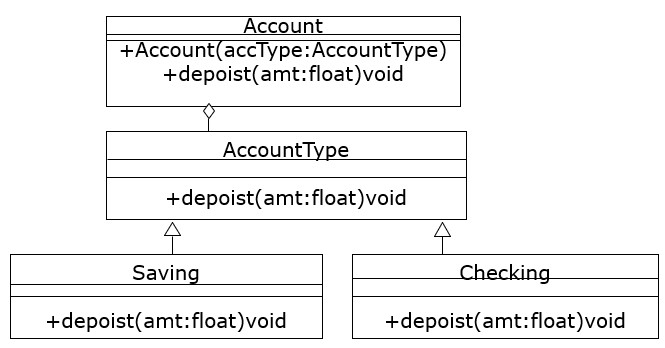
\includegraphics[width=0.55\textwidth]{12_1.jpg}
\end{figure}
\begin{lstlisting}[language=java]
// Account
Public class Account {
  private AccountType accountType;
  public Account(AccountType accType)
  {
    accountType=accType;
  }
  public void deposit(float amt)
  {
    accountType.deposit(amt);
  }
}
Account acc=new Account(new Checking());
\end{lstlisting}
\begin{lstlisting}[language=java]
// AccountType
abstract public class AccountType {
  public abstract void deposit(float amt);
}
\end{lstlisting}
\begin{lstlisting}[language=java]
// Saving
public class Saving extends AccountType {
  public void deposit(float amt) {
    //write your code here
  }
}
\end{lstlisting}
\begin{lstlisting}[language=java]
// Checking
public class Checking extends AccountType {
  public void deposit(float amt) {
    //write your code here
  }
}
\end{lstlisting}
在这个例子里,Account类依赖于AccountType这个抽象类型,而不是它的子类型。
AccountType有两个子类型:
\begin{itemize}
  \item 储蓄账号:以Saving具体类代表
  \item 支票账号:以Checking具体类代表
\end{itemize}
Account类并不依赖于具体类,因此当有新的具体类型添加到系统中时, Account类不必改变。
例如,如果系统引进了一个新型的账号:
MoneyMarket类型, Account类以及系统里面所有其他的依赖于AccountType抽象类的客户端均不必改变。其源代码如下:
\begin{lstlisting}[language=java]
public class MoneyMarket extends AccountType {
  public void deposit(float amt) {
    //write your code here
  }
}
\end{lstlisting}
\end{document}
